%% ------------------------------------------------------------------------- %%
\chapter{Conceitos}
\label{cap:conceitos}

Texto texto texto texto texto texto texto texto texto texto texto texto texto
texto texto texto texto texto texto texto texto texto texto texto texto texto
texto texto texto texto texto texto texto texto texto texto texto texto texto
texto texto texto texto texto texto texto texto texto texto texto texto texto
texto texto texto texto texto texto.

%% ------------------------------------------------------------------------- %%
\section{Fundamentos}\index{área do trabalho!fundamentos}
\label{sec:fundamentos}

Texto texto texto texto texto texto texto texto texto texto texto texto texto
texto texto texto texto texto texto texto texto texto texto texto texto texto
texto texto texto texto texto texto texto texto texto texto texto texto texto
texto texto texto texto texto texto texto texto texto texto texto texto texto
texto texto texto.

%% ------------------------------------------------------------------------- %%
\subsection{Ácidos Nucléicos}\index{ácido!nucléico}\index{nucleotídeos}
\label{sec:acidos_nucleicos}

Na Figura~\ref{fig:humanbeta} texto texto texto texto texto texto texto texto
texto texto texto texto texto texto texto texto texto texto texto texto texto
texto texto texto texto texto texto texto texto texto texto texto texto texto
texto texto texto texto texto texto texto texto texto texto texto texto texto
texto texto texto.

\begin{figure}[!h]
  \centering
  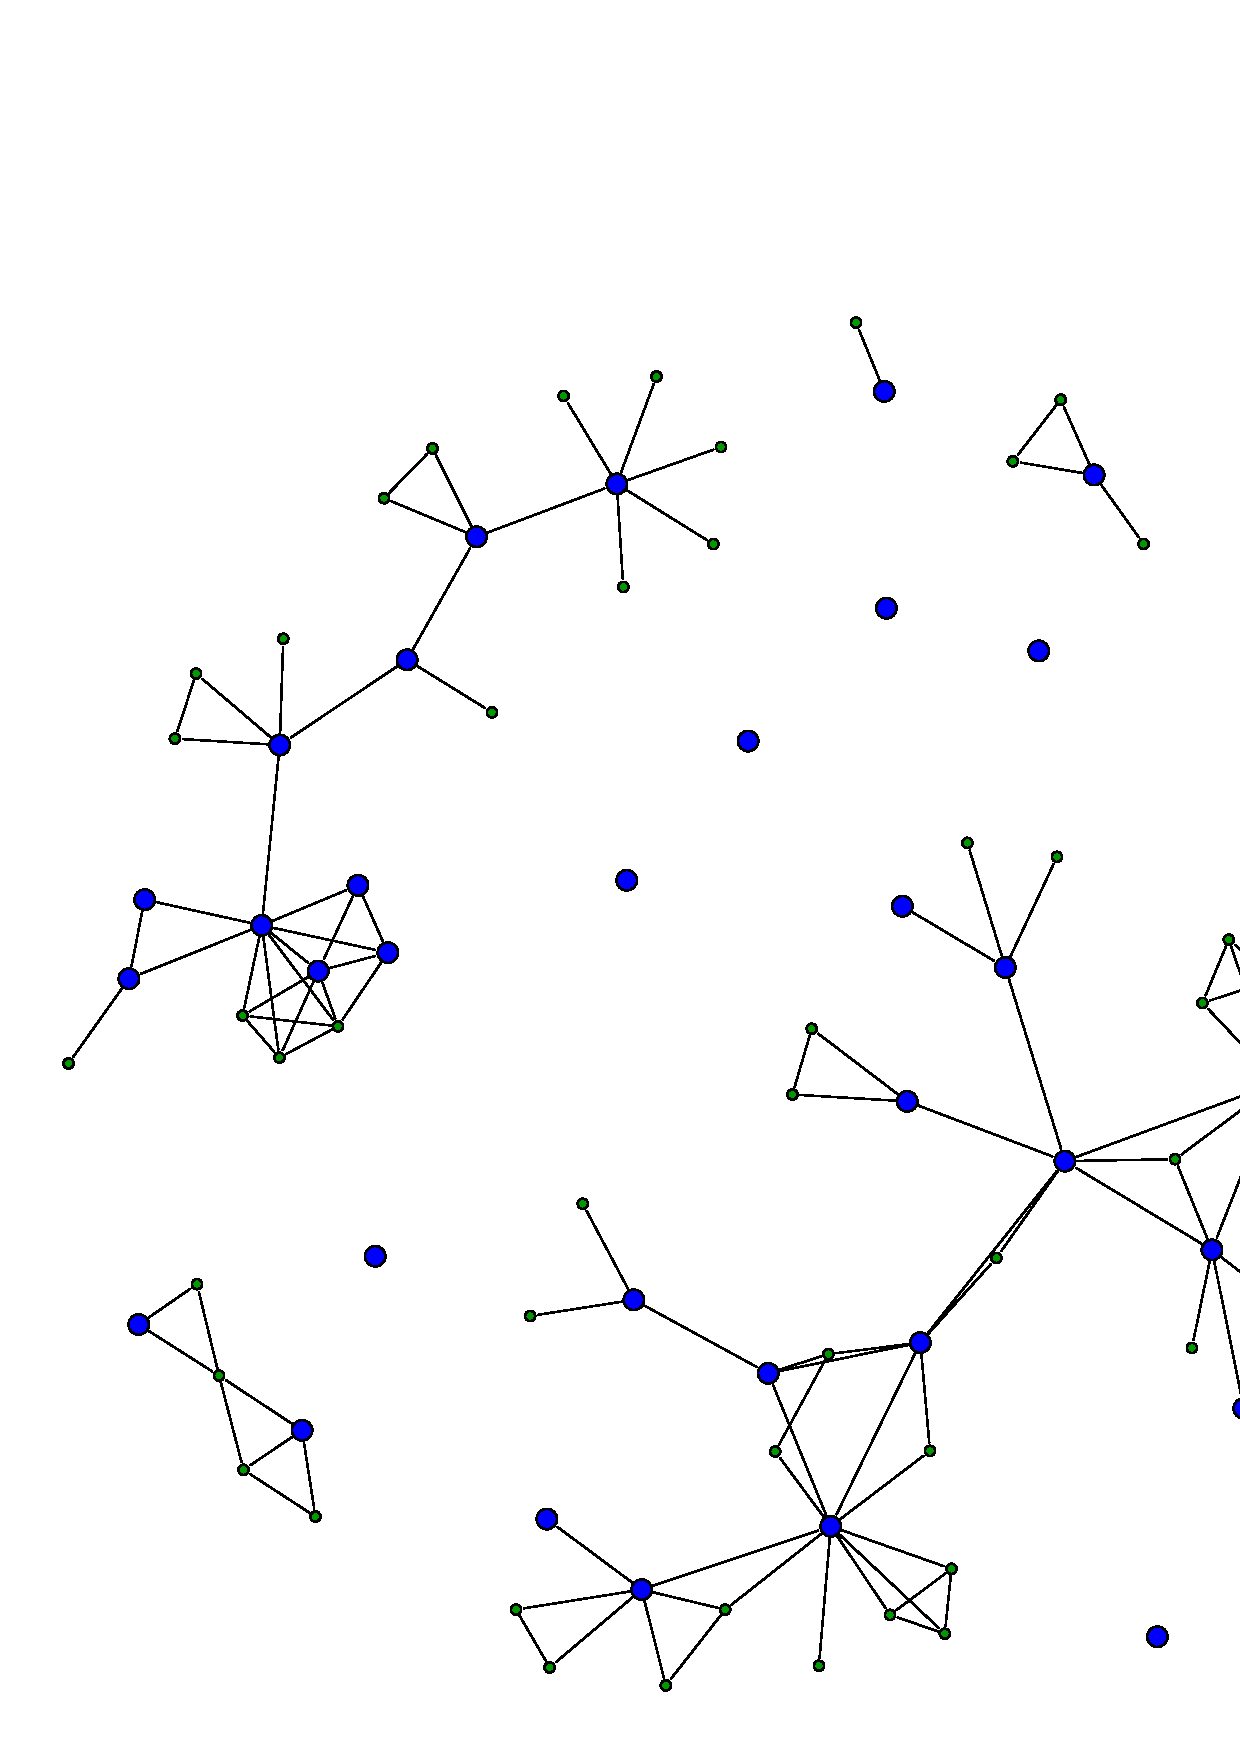
\includegraphics[width=.40\textwidth]{graph} 
  \caption{Descrição da figura mostrada.}
  \label{fig:humanbeta} 
\end{figure}

%% ------------------------------------------------------------------------- %%
\subsection{Aminoácidos}\index{ácido!amino|(}
\label{sec:amino_acidos}

Veja na Tabela \ref{tab:amino_acidos}...  texto texto texto texto texto texto
texto texto texto texto texto texto texto texto texto texto texto texto texto
texto texto texto texto texto texto texto texto texto texto texto texto texto
texto texto texto texto texto texto texto texto texto texto texto texto texto
texto texto texto texto texto texto texto texto texto texto texto.

\begin{table}[!t]
\begin{center}
    \begin{tabular}{c|c|l}
	 \hline
	 Código & Abreviatura & Nome completo \\ \hline
     \texttt{A} & Ala & Alanina \\
     \texttt{C} & Cys & Cisteína \\
     ...        & ... & ... \\
     \texttt{W} & Trp & Tiptofano \\
     \texttt{Y} & Tyr & Tirosina \\ \hline
    \end{tabular}
  \caption{Códigos, abreviaturas e nomes dos aminoácidos.}
  \label{tab:amino_acidos}
\end{center}
\end{table}
\index{ácido!amino|)}

Texto texto texto texto texto texto texto texto texto texto texto texto texto
texto texto texto texto texto texto texto texto texto texto texto texto texto
texto texto texto texto texto texto texto texto texto texto texto texto texto
texto texto texto texto texto texto texto texto texto texto texto texto texto
texto texto texto texto texto texto texto.


%% ------------------------------------------------------------------------- %%
\section{Exemplo de Código-Fonte em Java}
\label{sec:exemplo_codigo_fonte}
Texto texto texto texto texto texto texto texto texto texto texto texto texto
texto texto texto texto texto texto texto texto texto texto texto texto texto
texto texto texto texto texto texto texto texto texto texto texto texto texto
texto texto texto texto texto texto texto.

% Foi utilizado o pacote listing para formatar código fonte
% http://ctan.org/tex-archive/macros/latex/contrib/listings/listings.pdf
% Veja no preambulo do arquivo tese-exemplo.tex os parâmetros de configuração.

\begin{lstlisting}[frame=trbl]
    for(i = 0; i < 20; i++)
    {
        // Comentário 
        System.out.println("Mensagem...");
    }
\end{lstlisting}


%% ------------------------------------------------------------------------- %%
\section{Algumas Referências}
\label{sec:algumas_referencias}

É muito recomendável a utilização de arquivos \emph{bibtex} para o gerenciamento
de referências a trabalhos. Nesse sentido existem três plataformas gratuitas
que permitem a busca de referências acadêmicas em formato bib: 
\begin{itemize}
	\item \emph{CiteULike} (patrocinados por Springer): \url{www.citeulike.org}
	\item Coleção de bibliografia em Ciência da Computação: \url{liinwww.ira.uka.de/bibliography}
	\item Google acadêmico (habilitar bibtex nas preferências): \url{scholar.google.com.br}
\end{itemize}
Lamentavelmente, ainda não existe um mecanismo de verificação ou validação das
informações nessas plataformas. Portanto, é fortemente sugerido validar todas
as informações de tal forma que as entradas bib estejam corretas.  Também, tome
muito cuidado na padronização das referências bibliográficas: ou considere TODOS
os nomes dos autores por extenso, ou TODOS os nomes dos autores abreviados.
Evite misturas inapropriadas.

Exemplos de referências com a tag:
\begin{itemize}


\item @Article: \citep{MenaChalco08}.
{\scriptsize\begin{verbatim}
@Article{MenaChalco08,
 author   = {Jesús P. Mena-Chalco and Helaine Carrer and Yossi Zana and 
            Roberto M. Cesar-Jr.},
 title    = {Identification of protein coding regions using the modified 
            {G}abor-wavelet transform},
 journal  = {IEEE/ACM Transactions on Computational Biology and Bioinformatics},
 volume   = {5},
 pages    = {198-207},
 year     = {2008},
}
\end{verbatim}}


\end{itemize}

